\documentclass[conference]{IEEEtran}
\IEEEoverridecommandlockouts
% The preceding line is only needed to identify funding in the first footnote. If that is unneeded, please comment it out.
\usepackage{cite}
\usepackage{amsmath,amssymb,amsfonts}
\usepackage{algorithmic}
\usepackage{graphicx}
\usepackage{textcomp}
\usepackage{xcolor}
\usepackage{hyperref}
\usepackage{enumerate}
\usepackage{enumitem}
\usepackage{float}
\setlist[enumerate]{label*=\arabic*.}
\hypersetup{
    colorlinks=true,
    linkcolor=blue,
    filecolor=magenta,      
    urlcolor=cyan,
}
\def\BibTeX{{\rm B\kern-.05em{\sc i\kern-.025em b}\kern-.08em
    T\kern-.1667em\lower.7ex\hbox{E}\kern-.125emX}}
\begin{document}

\title{Survey and Taxonomy of Cyber Anomaly Detection Literature\
}

\author{\IEEEauthorblockN{1\textsuperscript{st} Wayne R. Havey III}
\IEEEauthorblockA{\textit{UCCS}\\
Colorado Springs, CO \\
whavey@uccs.edu}
}

\maketitle

\begin{abstract}
Detection papers can be categorized by their selection of a few key elements. The environment being monitored for anomalies, the type of anomaly being detected, the data needed to perform the detection, the methods used to perform analysis on that data, and specific tools to implement those methods. Additional surveys, taxonomies, and case studies can still fall under the proposed taxonomy. As far as the author knows there has been no single effort to classify detection papers using all of the above mentioned categories. This paper will provide a more complete classification for which a potential researcher, academic or professional, can use to classify detection literature. This classification can be used as an approach to determine if the researcher has done their due diligence in understanding and even implementing enough strategies to detect the gamut of anomalies. 
\end{abstract}

\section{Introduction}
In an ever increasing cyber landscape just like in any increasing population, the level of crime increases with it. Methods to detect crime vary by type. A detective doesn't use the same methods to track a serial killer as he or she does to track a petty thief. At a higher level, the united states doesn't enlist local police to detect threats to national security. The detective looks for different types of clues, asks different questions of different people, and will enlist different tiers of resources to help track down the suspect. The united states will enlist the CIA or FBI to hunt for national threats. The cyber "detective", should think in a similar fashion. That is; defining what exactly they are attempting to detect, the information that can be gathered from the susceptible environment, and the methods which can be applied to that information in order to detect anomalies. \\
At the highest level this papers goal is to assist the cyber detective; a security researcher, in being able to detect every type of cyber anomaly. Of course just as crime slips through undetected so do cyber anomalies. However just as a nation enlists the support of multiple entities with different skill sets (FBI, CIA, Police, Military, etc.) to attempt to catch every type of criminal, requirements should be defined for detecting as many types of cyber anomalies as possible. \\
To help address this issue this paper puts forth a classification model for detect literature. Using this classification a researcher can organize their reading to ensure all relevant detection topics are covered. Additionally, after enough papers are classified using this model gaps in research should become obvious.\\
The classification can be applied by answering a series of questions about the literature.

On a quick browse a researcher can answer the following three simple questions regarding the paper being read. 
\begin{itemize}
    \item What is being detected?
    \item What data is needed to perform that detection?
    \item What analysis methods are performed on the data to perform the detection?
\end{itemize}
Answering only these can still provide a mechanism for which a researcher may be able to see where there is more or less saturation in the field.

Breaking these three questions down further will provide greater insight and separate literature further.
\begin{itemize}
    \item Is a specific environment addressed?
        \begin{itemize}
            \item Are multiple environments addressed?
        \end{itemize}
    \item Is a specific type of attack addressed?
    \begin{itemize}
        \item Is only one type of attack addressed?
        \item Are multiple types of attacks addressed?
        \item Does the paper claim to address all anomalies, or anomalies in general?
        \begin{itemize}
            \item Does the behavior claim to detect malicious behavior, suspicious behavior, just anomalies, or some combination of these?
        \end{itemize}
        \item Does the paper focus on detecting advanced persistent threats (APT)?\\
        APTs have become such a widely studied and important topic that I believe it deserves to be separated out as a high level category.
    \end{itemize}
    \item Do the authors define the necessary data to collect in order to perform their detection method?
        \begin{itemize}
            \item Do the authors specify different data for detecting different anomalies?
            \item Do the authors focus on or specify a specific method of data organization?
        \end{itemize}
    \item What is the method the authors are using to perform the detection?
    \item Are the authors using a specific tool to implement the method of detection.
\end{itemize}
Of course many more sub-criteria may exist that can be used for further refinement but the above list contains the primary factors used to classify detection literature.
\\ It will be shown that taxonomies exist for each category presented and in some cases more than one. However, to the knowledge of the author there has been no single taxonomy put together that encompasses all of them and presents them in an order for which a researcher can follow a logical flow to categorize detection literature.

\section{The Classification}
Beginning with what to detect, define data needed, then define methods to perform analysis on the data, find specific tools to assist with implementation. Each step could be recursive. Researchers can classify their papers as well as others in the field. Gain insight into what detection methods are saturated, where gaps are, whether or not a paper has done a good job defining how to implement their proposed method and how well it does and detecting specific things. A fully monitored system(s) should be able to cover every attack type, thus defining every data source and method needed and tools that can assist. 

\section{Environments}
 There can be major differences in detection methodologies based on the type of environment. For example in cyber physical systems, such as the systems managing an electrical grid, there are very specific types of logs and highly tailored attacks. Whereas in a computer network comprising of tens or hundreds of hosts running one of several operating systems there are many types of data to collect, and many attack vectors to be aware of. Some methods may overlap but often times detection literature will specify if their proposed techniques are designed for detection in a specific environment. Agrawal et. al. propose a physics based method for detecting insider threats specifically in cyber physical systems\cite{agrawal2018poster}.
The proposed taxonomy puts forth a separation of detect literature based on the following environment types: Enterprise, Mobile, Cyber Physical Systems. Enterprise can be broken down further into: Windows, Linux, Mac, or combination.

\section{Attack Types}
\begin{figure}[h]
  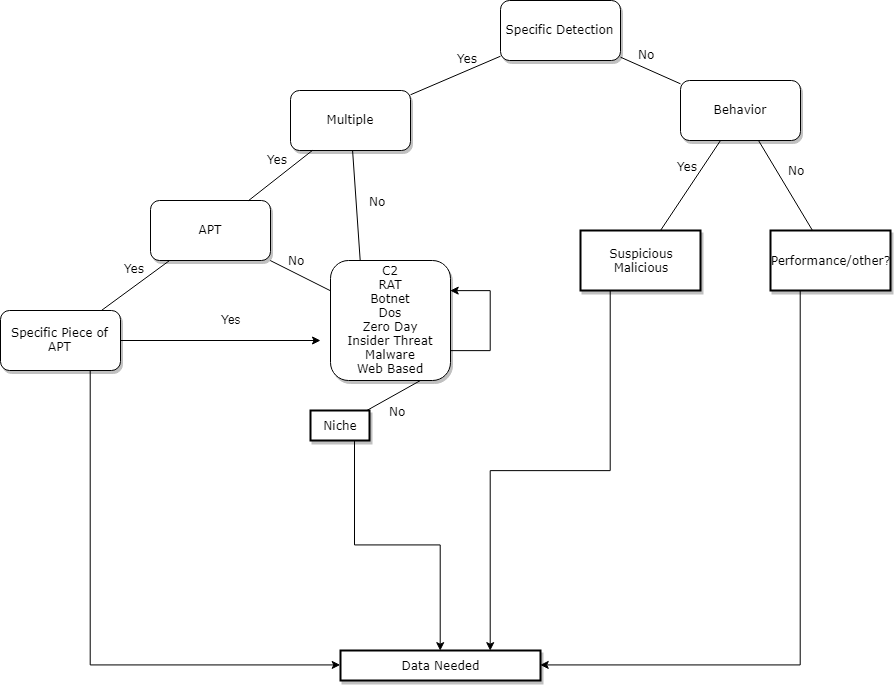
\includegraphics[width=.45\textwidth,height=6cm]{attack_types.png}
  \caption{Specific Detections}
  \label{AAA}
\end{figure}
This paper will puts forth a proposed sub taxonomy for classifying cyber anomaly types based on what was seen the most in surveying the literature. There are already several that exist that can be used for this section of the overall classification. Several surveys have already been written that address this topic. The Mitre "ATT\&CK" (Adversary Tactics Techniques and Cyber Killchain) framework may be appropriately be used here.  \cite{lazarevic2005intrusion}\cite{mitchell2014survey}\cite{axelsson2000intrusion}. Hansman et. el. propose an attack type taxonomy based attack vectors.
\cite{hansman2005taxonomy} \cite{hansman2005taxonomy} 
\begin{enumerate}
    \item Denial of Service (DOS) \cite{zargar2013survey}\cite{warrender1999detecting}\cite{lee1999data}
    \\The literature may even break DOS attacks down further.
    \begin{enumerate} 
        \item distributed
        \item CPU Exhaust
    \end{enumerate}
    \item Surveillance \& Probing \cite{lazarevic2005intrusion}
    \item C2 \cite{chen2014study}\cite{jasek2013apt}\cite{bhatt2014towards}
    \item Malware\cite{gabriel2009analyzing}\cite{tankard2011advanced}
    \\Malware is mentioned in the classification in terms of detecting its presence within the environment. Malware analysis techniques are outside the scope of this taxonomy.
    \item Web Based Attacks
    \item Embedded Systems Attacks
    \item Zero Days\cite{kotenko2012common}\cite{chen2014study}\cite{jeun2012practical}
    \item Side Channel Attacks
    \item Botnets\cite{singh2014big}\cite{awad2017network}
    \item Remote Access Trojans (RAT)\cite{wu2017detecting}
    \item Insider threats\cite{mukherjee1994network}
    \item Multiple or All
    \item APT\cite{jasek2013apt}\cite{saud2015towards}\cite{kim2013detection}
    \\APTs are often the primary focus of detection literature and typically use many attack types in their campaign from the above list. They are separated out here because detecting them is more involved than just detecting multiple attacks types.

\end{enumerate}

\section{Data to Collect}
\begin{figure}[h]
  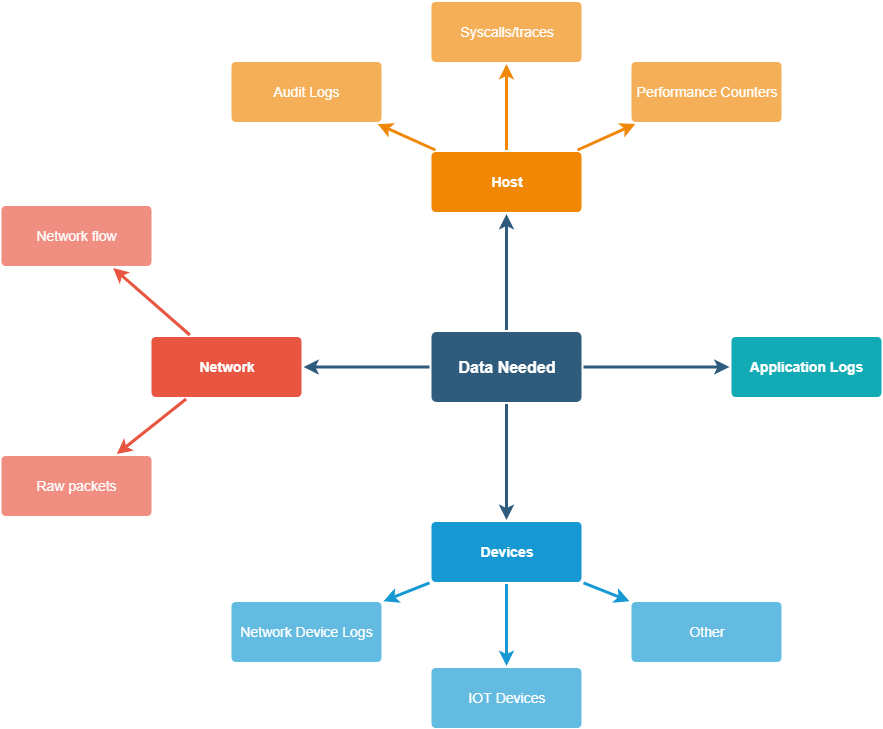
\includegraphics[width=.45\textwidth,height=6cm]{Data_needed.png}
  \caption{Data to Collect}
  \label{AAA}
\end{figure}
All good detection literature should specify the data that needs to be collected in order to perform the proposed detection method. If it is not specified it should be implicit what the source is or if all possible data sources be collected. Additionally, it is helpful for the literature to specify the collection mechanisms, storage strategy, and if relevant the retention period.  

Vendor specific, OS types. Understanding format, helpful to convert to specific format. Data types could be found within each other. Event IDs could potentially be another category.
\begin{enumerate}
    \item Host Logs\cite{jia2017big}\cite{marchetti2016analysis}
    \\Data in this category can be broken down further by operating system type.
    \begin{itemize}
        \item Windows
        \begin{itemize}
            \item Primary Example: Windows Event Logs
        \end{itemize}
        \item Linux
        \begin{itemize}
            \item Primary Example: Auditd logs
        \end{itemize}
    \end{itemize}
    \item Application Logs\cite{giura2012context}\cite{ten2010cybersecurity}
    \\Application Logs is a broad category.
        \begin{enumerate}
            \item agents\cite{garcia2009anomaly}
            \\Agents are a special type of software that are designed (in the context of this paper) to send security information to a system where specific events can be viewed by an analyst. There may be overlap between agents and the default logging mechanisms on the system but the agent is designed to collect specific information and forward it in a specific format.
            \item Honeypots and Canarys\cite{jasek2013apt}
            \\Honeypots are a special type of detection mechanism used to decieve an attacker typically used in conjunction with Canaries which are designed to immediately alert an analyst upon their access or the access of data around them. Honeypot and canary data may come in various formats although typically in the form of network traffic. It is worth separating them from standard network based data because they provide such a specific function. 
        \end{enumerate}
    \item System calls (syscalls) \cite{warrender1999detecting}\cite{hofmeyr1998intrusion}
    \item Device Logs\cite{horne2002management}
    \begin{enumerate}
        \item Network devices
        \begin{itemize}
            \item Routers
            \item Switches
            \item Firewalls
        \end{itemize}
        \item Internet of Things (IOT) devices
        \item Mobile devices
    \end{enumerate}
    \item Network flow \cite{kim2013detection}
    \begin{itemize}
        \item Raw packets
        \item Network flow data
    \end{itemize}
    \item Performance Counters
\end{enumerate}

\section{Detection Methods}
This is the real meat of cyber anomaly detection literature and so comprises the most critical and easily determined part of the taxonomy. Many of the categories presented here can and have been broken down much further in other surveys. It is recommended that for a deeper classification other surveys are explored in conjunction with what is presented below. With that said, there will be breakdowns of the categories presented here representing the most commonly observed detection strategies in the papers analyzed for this survey.

Ever growing, Automation, Hybrids, Analyst training and understanding the human factor. Alerting.
\begin{enumerate}
    \item Machine Learning\cite{buczak2016survey}\cite{dua2016data} 
    \begin{enumerate}
        \item Training\\
        It has been observed that a large amount of detection literature focusing on machine learning techniques make use of the Darpa data set for training. 
        \item Algorithms
        \begin{enumerate}
            \item Random Forest \cite{singh2014big}
            \item K-means\cite{asif2011filtering}\cite{hajamydeen2016unsupervised}
        \end{enumerate}
        \item clustering \cite{asif2011filtering}   
        \item classifying
        \item Regression analysis
    \end{enumerate}
    \item Analytics\cite{cardenas2013big}
    \item Attack Graphs\cite{abraham2015predictive}
    \item Data Organization
    \\ Data organization was briefly mentioned in the data collection portion of the taxonomy. However, some literature in the field place a high importance on the the organization of being in itself a method for detection.
    \item Architecture
    \\ Similar to data organization the architecture of the detection system provides in itself a means for detecting cyber anomalies.
    \item Query Languages\cite{mukherjee1994network}
    \\ Query languages present an interesting detection mechanism that is heavily related to analytics as they provide a means for them to be created them on the fly. Because of this, their effectivness is likely correlated with the skill and knowledge of the analyst. This may be an interesting research topic.
    \item Behavior definition
    \item Tagging
    \item Honey Tech \cite{jasek2013apt}\cite{saud2015towards}
    \item White Lists\cite{yen2013beehive}
    \item Temporality\cite{abraham2015predictive}\cite{abraham2014cyber}
    \item Algorithms\cite{kim2013detection}
\end{enumerate}
\section{Tools}
This subsection is less commonly observed in detection literature and truthfully less important. It can provide insight into how a particular method can be perform better with a particular tool. In some cases the tool is a primary focus of the literature and so the author believes it is still necessary to include in the taxonomy. Similar to other categories the tools listed here are representative of what was most commonly observed in the literature studied for this survey. At a higher level the tool classification can be broken down into Recently used, popular, and novel. A potential use case for adding this level of classification is to see what methods a tool is not being used for that it potentially could be.
\begin{enumerate}
    \item SIEM \cite{kotenko2012attack}
    \item Weka \cite{asif2011filtering}\cite{thevar2017effect}
    \item Spark \cite{gupta2016framework}\cite{dobson2018performance}
    \item Hadoop \cite{gupta2014big}\cite{tankard2012big}
    \item Commercial 
\end{enumerate}

\section{The Classification as a Logic Diagram/FSM/automaton/flow chart?}
\section{Applications}
\subsection{In Research}
Future research could apply model as figure in paper so quick scan reveals their goal. Classification of enough literature could reveal where research is lacking, stale, old, or over-saturated. 
\subsection{In Development and Testing}
Model applied to define requirements for a monitoring platform. Could be applied to define tests. Ensure analytics created for everything. Comparison of tools. Define analyst training.

\Section{Potential Future Work}
Providing an application for literature classified using the proposed taxonomy that can be easily searched. Defining response mechanisms for permutations of of the taxonomy.

\begin{figure*}
  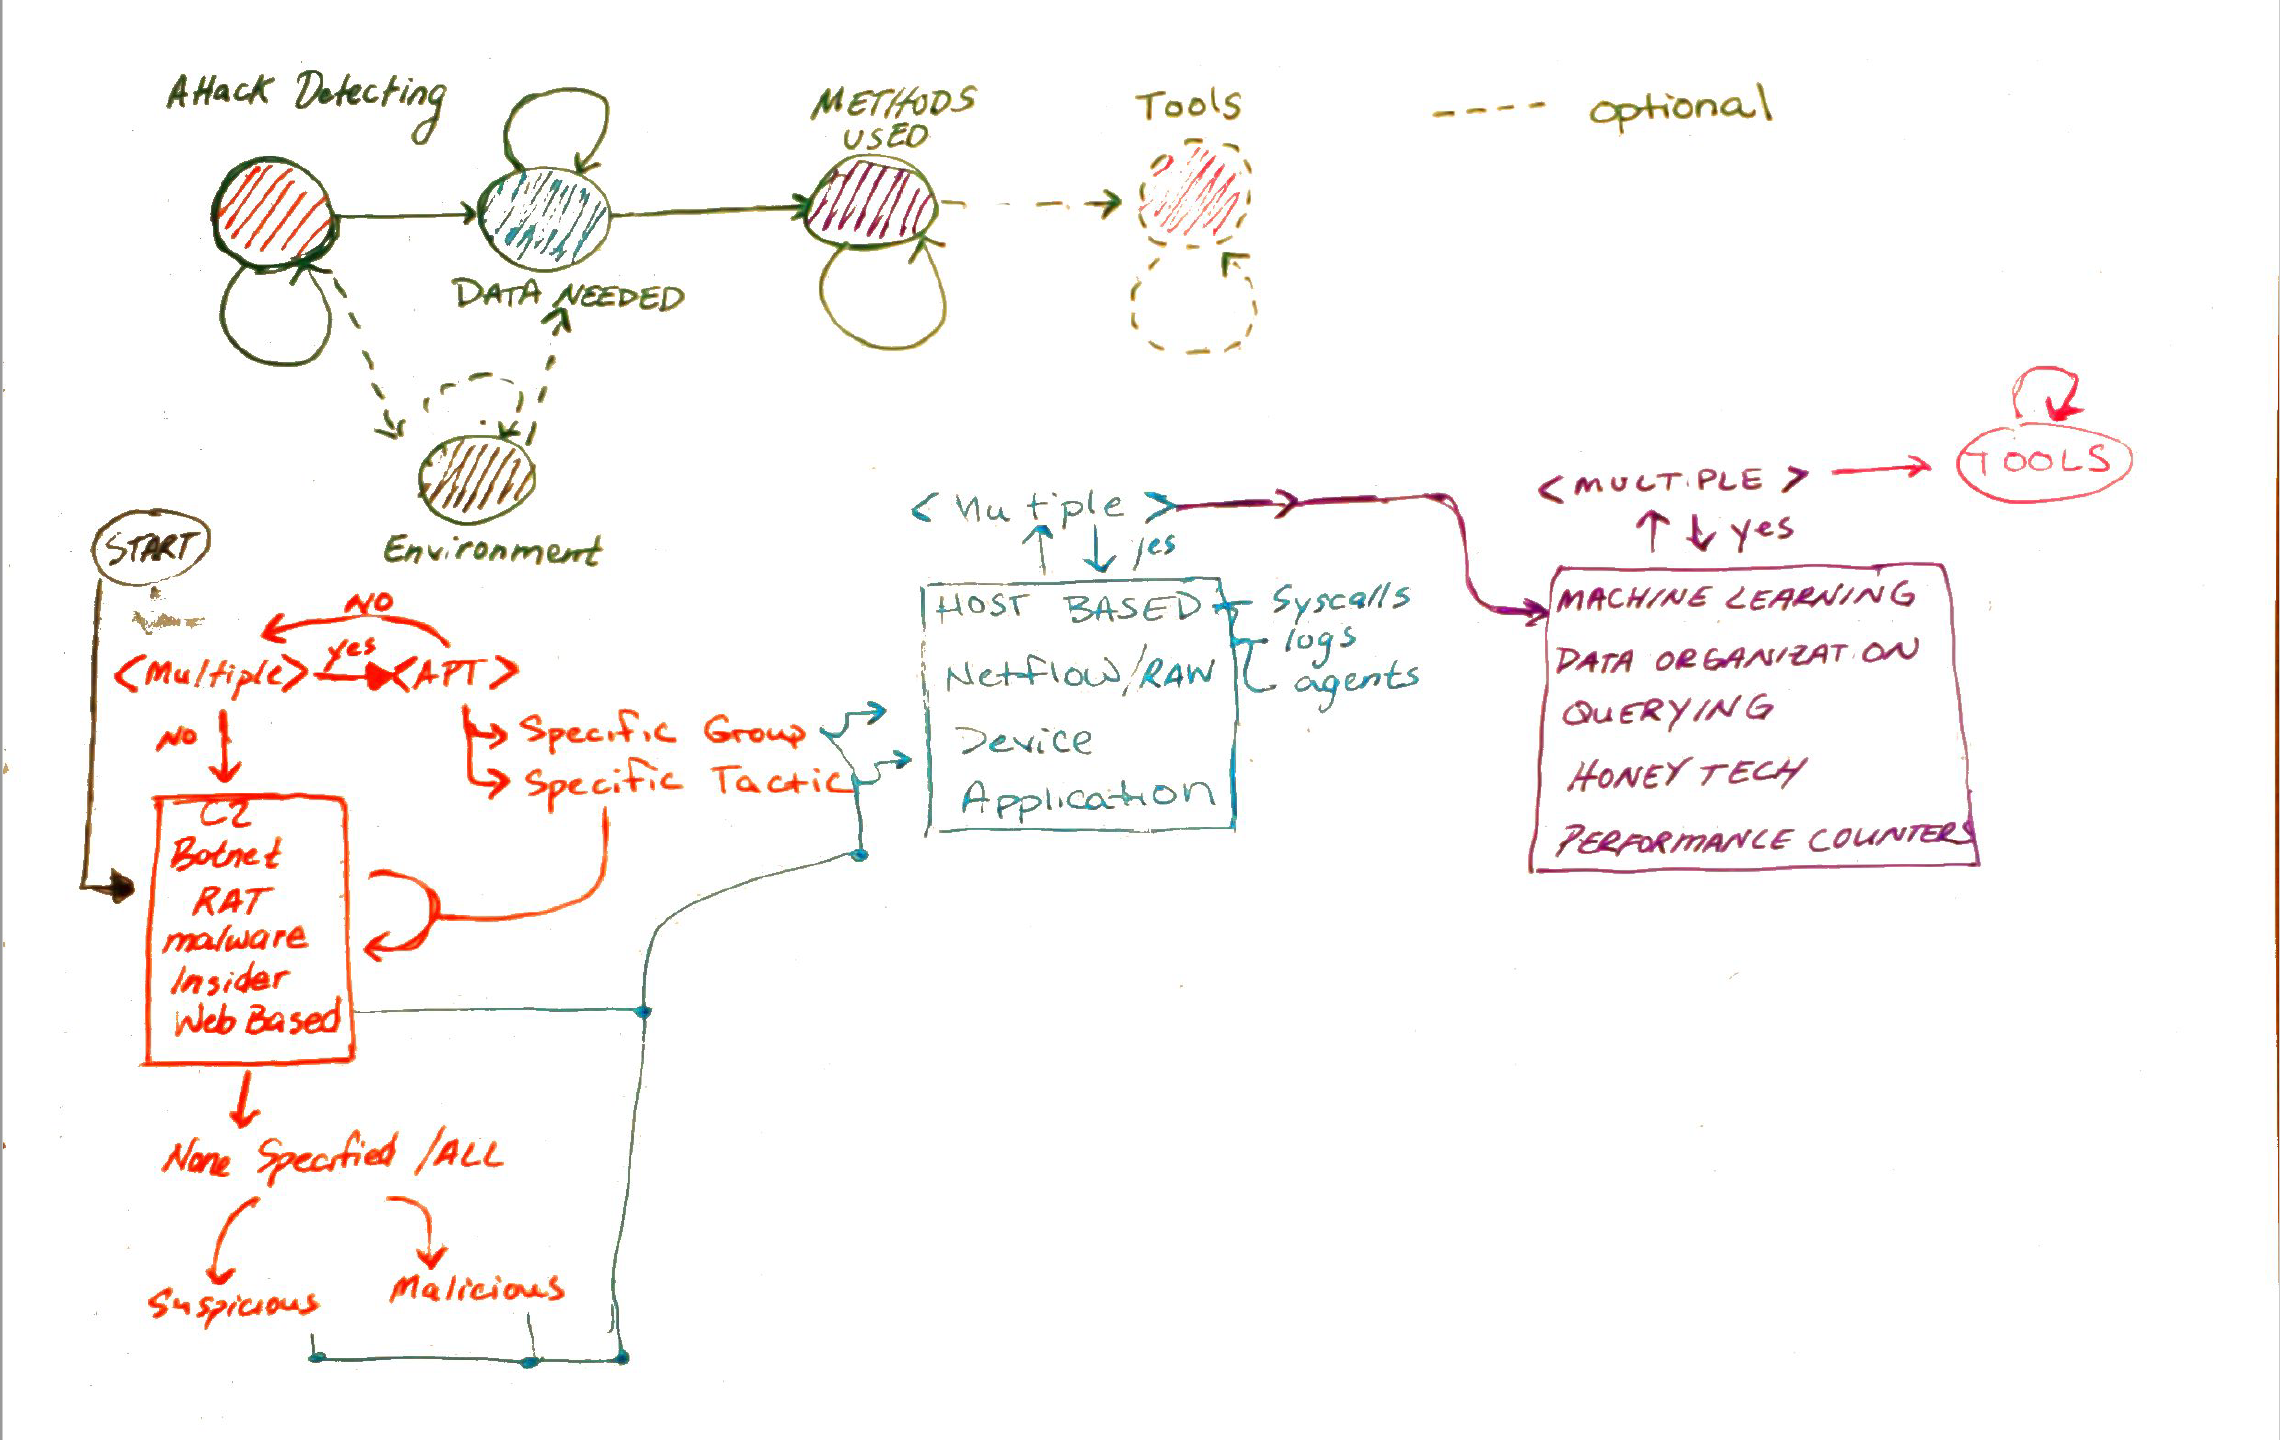
\includegraphics[width=\textwidth,height=10cm]{hwdiag.png}
  \caption{Classification Model}
  \label{AAA}
\end{figure*}
\section{Paper List}
\begin{enumerate}
    \item 
    PERFORMS: Machine Learning (Naive Bayes and frequent sequence algorithm) \\ 
    ON: Network flow data\\ 
    DETECTING: RATs 
    \cite{wu2017detecting} 
    \item 
    PERFORMS: multiple data modeling methods (defining normal behavior)\\ 
    ON: system calls\\ 
    DETECTING: abnormal behavior 
    \cite{warrender1999detecting}
    \item  
    PERFORMS: Machine learning\\ 
    ON: Web server logs (application logs e.g apache)\\ DETECTING: Web based attacks 
    \cite{kruegel2003anomaly}
    \item 
    PERFORMS:Machine learning - classification (k-nearest neighbors)\\ 
    ON: Netflow data (streamed)\\ 
    DETECTING: Attacks - DOS,User to root, remote to local,Probing\\ 
    USING: Apache Spark 
    \cite{thevar2017effect} 
    \item 
    PERFORMS: Data analysis algorithm (analytics)\\ 
    ON: Network Flow data (ingress \& egress points),Email logs,syslog (privesc)\\ 
    DETECTING: APT \cite{kim2013detection} 
    \item 
    PERFORMS: Machine Learning\\ 
    ON: Multisource\\ 
    DETECTING: Abnormal Behavior\\ 
    USING: spark 
    \cite{jia2017big} 
    \item 
    PERFORMS: Machine Learning (Markov Chain building normal profile)\\ 
    ON: audit data (unix)\\ 
    DETECTING: Abnormal Behavior \cite{ye2004robustness}
    \item 
    PERFORMS: Machine Learning (random forest)\\ 
    ON: Network flow data\\ 
    DETECTING:Botnets (p2p)\\ 
    USING: mahout, hadoop, HIVE 
    \cite{singh2014big}
    \item 
    PERFORMS: Analytics (not very in depth)\\ 
    ON: Web Server (application) logs\\ 
    DETECTING: Insider threat 
    \cite{myers2009towards}
    \item 
    PERFORMS: Analytics (not well defined)\\ 
    ON: Multisource (firewall,netflow, not well defined)\\ DETECTING: APT/Zero Days \cite{ahn2014big} 
    \item 
    PERFORMS: Machine Learning\\ 
    ON: Performance Counters\\ 
    DETECTING: Malware 
    \cite{demme2013feasibility}
    \item 
    PERFORMS: ML Classification\\ 
    ON: Binary metadata\\ 
    DETECTING: New malware binaries (windows) \cite{schultz2001data}
    \item 
    PERFORMS: analytics\\ 
    ON: Netflow data\\ 
    DETECTING: probing, suspicious behavior\\ 
    USING: honeypot/net \cite{hieb2004anomaly}
    \item 
    PERFORMS: Vulnerability Analysis and Attack Graph Analysis\\ 
    ON: nessus data (application), host logs, network device logs (not well defined)\\ 
    DETECTING: malicious behavior \cite{jajodia2009topological}
    \item 
    PERFORMS: novel query language\\ 
    ON: multiple source logs (not well defined)\\ 
    DETECTING: malicious behavior \cite{gao2018saql}
    \item 
    PERFORMS: New architecture (embedded systems) performing analytics real time\\ 
    ON: syscall data\\ 
    DETECTING: Malicious execution \cite{rahmatian2012hardware}
    \item 
    PERFORMS: Data organization, feature extraction, Machine learning (clustering k-means)\\ 
    ON: Multisource logs (well defined)\\ 
    DETECTING: Suspicious (specifically states only suspicious)\\ 
    USING: SIEM \cite{yen2013beehive}
    \item 
    PERFORMS: ML (supervised learning)  \\
    ON: API calls  \\
    DETECTING: Zero-day malware \\
    \cite{alazab2011zero}
    \item
    PERFORMS: Analytics (normal behavior) \\
    ON: Performance Counters (branch miss predictions, instruction TLB (iTLB) misses and L2 cache misses, very well defined) \\
    DETECTING: Code-injection, return to libc, return oriented programming attacks (very well defined)  \\
    USING: Novel tool Eumonia 
    \cite{yuan2011security}
    \item
    PERFORMS:  ML (TCM-KNN)\\
    ON: netflow, application (bro) \\
    DETECTING: mutliple attack types (very well defined: Probes, DoS (Denial of Service), U2R (User to Root) and
R2L (Remote to Local))
    \cite{li2007network}
    \item
    PERFORMS: Machine Learning (2 Anomaly detection, supervised learning) (analytics: correlation of l3 cache misses b/t 2 processes)  \\
    ON: Performance Counters  \\
    DETECTING: Cache Based Side Channel Attacks (in title) (flush and reload) 
    \cite{chiappetta2016real}
    \item
    PERFORMS: Attack modeling data organization \\
    ON: Specifically states ALL data collectable \\
    DETECTING: APT
    \cite{giura2012context}
    \item
    PERFORMS: Generic honeypot Alerting \\
    ON: netflow data \\
    DETECTING: APT \\
    USING: KFSensor
    \cite{saud2015towards}
    \item
    PERFORMS: ML  \\
    ON: Temporal Netflow data (bro)  \\
    DETECTING: U2R, R2L, DOS, Probing
    \cite{lee1999data}
    \item
    PERFORMS: Special Architecture, event correlation (analytics)  \\
    ON:  Multisource log data\\
    DETECTING:  APT
    \cite{bhatt2014towards}
    \item
    PERFORMS: Data organization and ML \\
    ON: States multisource (appears to be mostly netflow data from applications)  \\
    DETECTING: anomalies
    \cite{hajamydeen2016unsupervised}   
    \item
    PERFORMS: Temporal data organization (multiple methods compared)  \\
    ON: Alerts \\
    DETECTING: anomalies
    \cite{pierazzi2016exploratory}
    \item
    PERFORMS: ML,DeepL,nueral net,  \\
    ON: multisource logs \\
    DETECTING: cyber anomalies
    \cite{du2017deeplog}
    \item
    PERFORMS: ML Markov Chain Model  \\
    ON: Binary data \\
    DETECTING: ROP chaining 
    \cite{usui2016poster}
    \item
    PERFORMS: Graphing, ML classification \\
    ON: System and Network level events (not well defined) \\
    DETECTING: Malware Downloads
    \cite{rahbarinia2016real}
\end{enumerate}

\bibliographystyle{IEEEtran}
\bibliography{survey_bibtex}
\end{document}